\chapter{Theory}

\section{Feature extraction}

\textbf{by Paul Warkentin} \\

The state of the art method for feature extraction from audio for speech recognition purposes is to use Mel Frequency Cepstral Coefficients (MFCC). They were introduced in 1980 by Davis and Mermelstein, and the European Telecommunications Standards Institute (ETSI) defined a standardised MFCC algorithm to be used in mobile phones. \\
Based on the underlying assumption, that audio frequencies change very little over very short intervals of time, the signal is divided into 10ms intervals. For each interval, a sequence of transformations is applied, resulting in 13 coefficients.

% TODO: more about MFCC mechanism

MFCC can be used to identify all the parts of the audio that belong to linguistic content and distinguish these from those parts in the audio signal which carry information about silence, background noise, laughter etc.

\section{Classification}

\textbf{by Paul Warkentin} \\

The main part of this project is the classification of extracted audio signals of linguistic content. This is a typical problem in the field of speech recognition, for which convolutional neural networks are a widely used class of deep, feed-forward artificial neural networks. \\
An important feature of convolutional neural networks is that they are translation invariant. The input data for our model are intervals containing MFCC datapoints. Because we do not know where in the interval the features which determine the word being said are localized, the shift invariance feature of convolutional neural networks is ideal for the speech recognition part in our problem.

% For speech recognition, convolutional networks are a widely used form of deep learning models. That is why we built our graph using two convolutional layers, followed by ReLU layers. The output of the first ReLU layer is also pooled. At the end, the output of the second ReLU layer is transformed by two dense layers into the result of the model.

% \begin{figure}
%     \centering
%     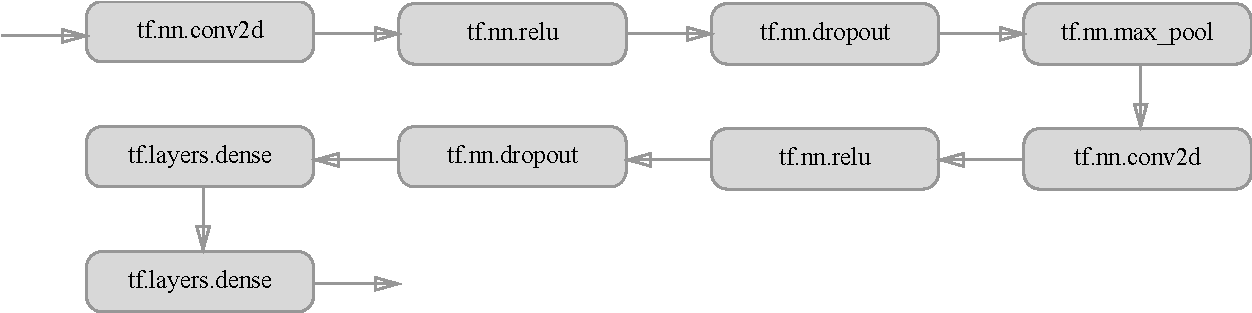
\includegraphics[width=\textwidth]{\RootPath/graphics/graph}
%     \caption{Classifier}
% \end{figure}
